\section{Responsive Web} \label{sect:responsive-web}

지금까지 CSS를 이용하여 문서를 디자인하는 방법을 다루면서 주로 가로 폭이 넓은, PC의 웹 브라우저를 기준으로 작업해왔다. 그러나 모든 사용자가 웹 페이지를 항상 PC와 같이 가로 폭이 넓은 디바이스에서 열람하는 것은 아니다. 휴대폰과 같은 모바일 디바이스는 가로 폭이 좁기 때문에, PC를 기준으로 설계한 웹 페이지는 모바일에서 열람했을 때 가독성이 심각하게 저하될 수 있다. HTML 요소들이 의도와는 다르게 배치될 수 있고, 이를 방지하고자 요소의 너비 등을 정해진 값으로 딱딱하게 정하면 모바일 디바이스에서는 좌우로 스크롤하면서 웹 페이지를 읽어야 합니다. 웹 페이지는 가급적 좌우 방향으로는 움직이지 않고, 상하 방향으로만 움직여 정보를 전달하게끔 설계하였을 때 가독성이 좋은데, 위와 같이 PC를 기준으로 웹 페이지를 설계하면 가독성이 매우 떨어진다. 따라서, 웹 페이지가 렌더링되는 화면의 크기에 따라 디자인이 바뀌는, \textbf{반응형 웹 페이지(Responsive Web)}를 디자인할 필요가 있다.

\begin{figure}[htb]\vspace{10pt}\centering
    \begin{subfigure}{.757\textwidth}\centering
        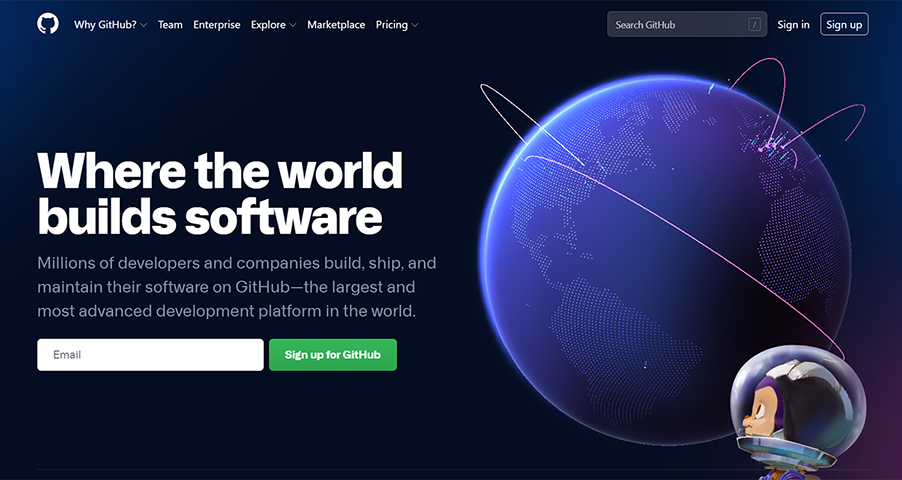
\includegraphics[width=\textwidth]{images/css-designing-html/github-responsive-desktop.png}
        \caption{Desktop Browser}
        \label{fig:github-responsive-desktop}
    \end{subfigure}
    \begin{subfigure}{.2\textwidth}\centering
        
\includegraphics[width=\textwidth]{images/css-designing-html/github-responsive-mobile.png}
        \caption{Mobile Browser}
        \label{fig:github-responsive-mobile}
    \end{subfigure}
    \caption{Webpage view of GitHub Homepage}
    \label{fig:github-responsive}
\end{figure}

\subsection*{Viewport}
반응형 웹 페이지는 웹 페이지가 렌더링되는 화면, 즉 뷰포트에 따라 디자인이 바뀌므로 먼저 뷰포트를 설정해주어야 한다. 뷰포트의 크기는 \coderef{code:viewport-setting}과 같이 HTML 문서의 \texttt{meta} 태그에서 설정한다.

\begin{codeenv}{code:viewport-setting}{Viewport Setting}\begin{verbatim}


<meta name="viewport" content="width=device-width, initial-scale=1" >
\end{verbatim}
\end{codeenv}

\coderef{code:viewport-setting}의 코드는 페이지의 너비를 디바이스 화면의 너비로 설정(\texttt{width=device-width})하고, 원래 페이지의 크기를 그대로 사용(\texttt{initial-scale=1})하는 코드이다. 이 코드가 가장 기본적인 설정이며, 추가 설정이 가능하다. 이러한 뷰포트 설정은 \sectref{sect:basic-structure-of-html}의 \coderef{code:html-example}에서도 확인할 수 있다.

뷰포트는 개발자 도구를 이용하여도 조절할 수 있다. Chrome의 경우 개발자 탭에서 Elements 탭 왼쪽에, Firefox의 경우 오른쪽 상단에 모바일 디바이스와 유사한 아이콘(Toggle device toolbar)을 눌러 뷰포트를 조절할 수 있다.

\subsection*{Media Query}
이제 CSS를 이용하여 웹 페이지를 반응형으로 디자인해보자. 반응형 웹페이지를 디자인하기 위해서 \texttt{@media query}라는 구문을 사용한다.

\begin{codeenv}{code:media-query-stmt}{Media Query Statement}\begin{verbatim}


@media only screen and (min-width: 800px) {
    /* CSS code goes here */   
}
\end{verbatim}
\end{codeenv}

\coderef{code:media-query-stmt}은 \texttt{@media query} 구문의 예시이다. 중괄호 내부에는 일반적인 CSS 코드를 작성하고, \texttt{@media query} 구문은 중괄호 내부의 디자인을 적용할 조건을 제시한다. 코드에서 \texttt{min-width: 800px}은 화면의 ``너비가 800px 이상''이라는 조건이며, 이 외에도 다양한 조건을 제시할 수 있으나 \coderef{code:media-query-stmt}이 가장 기본적인 형태이다.

\texttt{@media query} 구문을 이용하여 반응형 웹페이지를 디자인할 때 너비가 작은 화면에서 큰 화면의 순서로 작성하는 것이 원칙이다. 예를 들어, 뷰포트의 너비가 (1) 400px 미만일 때, (2) 400px 이상 800px 미만일 때, (3) 800px 이상 1200px 미만일 때, (4) 1200px 이상일 때의 디자인을 각각 다르게 설계하는 상황을 가정해보자. 먼저 (1)의 디자인을 먼저 작성하고, (2)의 디자인 중 (1)과 다른 부분을 \texttt{@media query} 구문을 이용하여 400px 이상의 뷰포트에 대해 작성한다. 이렇게 작성하면 (1)에서 작성한 디자인 중 (2)에 의해 덮어씌워지지 않는 디자인은 그대로 유지된다. (3), (4)도 마찬가지의 방법으로 작성하여 완성한다.
